\documentclass{article}

\usepackage{graphicx}
\usepackage{caption}
\usepackage{subcaption}
\usepackage[letterpaper]{geometry}
\title{Deep Belief Networks}
\date{2017-04-04}
\author{Nathan Zabriskie}

\begin{document}
	
	\maketitle
	
	\section{Introduction}
	For my deep learning project I decided to experiment with deep belief networks. I chose this model because I wanted to see what started the whole deep learning craze and I was especially interested in the generative capabilities of these networks. In this paper I will outline what experiments I performed and what I learned about the strengths and weaknesses of this model.
	
	\section{Implementation}
	In order to better understand how this model works I first implemented the algorithm by hand in C++. I originally had some trouble deciding how to effectively store the weights for each layer as they need to be readily available for backward passes in addition to the normal forward pass of a MLP. Once I realized that I should be treating each pair of layers as one restricted Boltzmann machine with one set of weights rather than two separate layers this problem solved itself. In my final implementation each pair of layers is treated as an RBM with the hidden nodes of one RBM acting as the visible nodes of the next RBM.
	
	 Once I was satisfied that my implementation was working I began experimenting with it only to find that it was incredibly slow, taking several hours to run over the MNIST dataset with a relatively shallow network of 4 layers total. I wanted to have time to do a variety of experiments so I ended up learning to use Tensorflow and reimplementing the model using that library. My Tensorflow implementation ran the same model over the same dataset in a matter of minutes rather than hours which made it much easier to test different hyperparameters and measure their effects. 
	
	\section{Experiments}
	I performed my experiments on the MNIST dataset. I chose this dataset because it is well studied and small enough in scope that I could run several experiments without having to train my network for days each time. In each experiment training stopped when validation set accuracy did not improve for a fixed number of epochs and final accuracy was measured for a test set using the weights which resulted in the highest validation set accuracy.
	
	\subsection{Baseline}
	To get some results to compare my DBN against I first ran the MNIST dataset through a MLP with 150 hidden nodes using relu activations and an output layer using softmax activations. This simple model performed surprisingly well averaging $\approx 98\%$ final accuracy for several runs. Decreasing the number of hidden nodes had a definite negative impact on the final test accuracy but increasing the number of hidden nodes past this point did not have a noticeable effect on the final test accuracy. Some runs would do better than others but this is simply due to the random splitting and shuffling of the training, validation, and test sets.
	
	\subsection{Deep Belief Networks}
	After getting some preliminary results I started experimenting with various hyperparameters in my DBN to determine their effects and to try to beat the accuracy of the baseline model. For each experiment validation set accuracy was measured once per epoch and training ended when the best validation accuracy did not improve for a set number of epochs. 
	
	During pretraining each RBM layer went through a fixed number of RBM updates before moving on to the next layer. Each RBM layer always output the sampled probabilities of the hidden layer rather than the probabilities themselves during pretraining but during actual training they could output either value.
	
	\subsubsection{Freezing RBM Layers}
	In this experiment I used a network with 4 RBM layers with (600,625,650,600) hidden nodes and one fully-connected output layer. After the initial pretraining the RBM layers were all frozen so the entire system only had 6010 trainable weights going from the final RBM layer to the outputs. 
	
	These restrictions had a significant impact on the overall accuracy dropping it from 98.1\% for the unfrozen network to 95.3\% for the frozen one. In this situation the system simply does not have enough degrees of freedom to accurately capture the features it needs to; I was actually surprised it did as well as it did. Adding another fully connected layer with 200 nodes brought the accuracy back up to 97.4\% but this is about equivalent to unfreezing a single layer so it is not that surprising.

	\begin{figure}[h!]
		\centering
		\begin{subfigure}[b]{0.4\textwidth}
			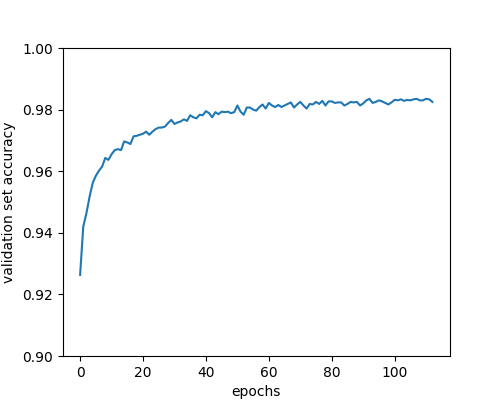
\includegraphics[width=\textwidth]{images/pretrain.png}
			\caption{With pretraining}
			\label{fig:pretrain}
		\end{subfigure}
		~
		\begin{subfigure}[b]{0.4\textwidth}
			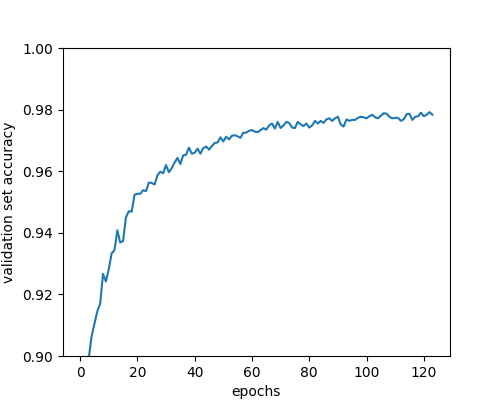
\includegraphics[width=\textwidth]{images/no_pretrain.png}
			\caption{Without pretraining}
			\label{fig:no_pretrain}
		\end{subfigure}
		\caption{Effects of pretraining on validation accuracy.}
		\label{fig:pretrain_comp}
	\end{figure}

	\subsubsection{Effects of Pretraining}
	After seeing the effects of freezing the RBM layer weights I wanted to see if pretraining the Boltzmann layers had any advantage over just randomly initializing the weights and learning them from the start.
	Figure \ref{fig:pretrain_comp} shows the results of an experiment where I ran an identical network two times. For the first run I did the normal DBN pretraining before moving into normal back propagation. In the second run no pretraining was performed and weights were initialized with a zero-mean Gaussian distribution before being trained. 	
	
	Although the final accuracy for each run was about the same, the plots do show some differences. When pretraining was performed the network was able to achieve $>92\%$ accuracy at the end of the first epoch whereas without pretraining it only had $45.1\%$ accuracy at the same epoch. In addition, the preconditioned network trained in less epochs than the randomly initialized network although it took more time overall when accounting for the time it took to precondition it.
	
	
	 
	\subsubsection{Generation}
	As I mentioned above, part of the reason I wanted to implement this particular model is because of its generative capabilities. In my first generative experiment I selected random training images, fed them forward through all the RBM layers of the network, then took the output of the last hidden layer and fed it backwards through all the previous layers to get a new image. In general, passing an image through the network in this way seems to have a blurring effect on the image similar to a Gaussian filter as shown in figure \ref{fig:regenerated}. I also noticed that the network was able to recreate some numbers better than others based on their complexity and curvature. Ones and sevens looked pretty good whereas it seemed to struggle creating recognizable twos, eights, and sixes.    
	
	\begin{figure}[h]
		\centering
		\begin{subfigure}[b]{0.3\textwidth}
			\centering
			
\includegraphics[scale=2.0]{images/in0}
			\caption{Input Image}
		\end{subfigure}
		\begin{subfigure}[b]{0.3\textwidth}
			\centering
			
\includegraphics[scale=2.0]{images/gen0}
			\caption{Regenerated Image}
		\end{subfigure}
	
		\begin{subfigure}[b]{0.3\textwidth}
			\centering
			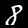
\includegraphics[scale=2.0]{images/in1}
			\caption{Input Image}
		\end{subfigure}
		\begin{subfigure}[b]{0.3\textwidth}
			\centering
			
\includegraphics[scale=2.0]{images/gen1}
			\caption{Regenerated Image}
		\end{subfigure}
	
		\caption{Regenerated images.}
		\label{fig:regenerated}
	\end{figure}

	In the second generation experiment I began by pretraining all the RBM layers and then creating a random vector sampled from a uniform distribution ranging from 0 to 1. This vector was then fed into the hidden layer of the last RBM and relaxed for k iterations before being fed backwards through the rest of the layers and output at the first visible layer. In general about 50\% of the images generated this way were recognizable while the other 50\% were severely distorted and disjointed. 
	
	\begin{figure}[h]
		\centering
		\begin{subfigure}[b]{0.2\textwidth}
			\centering
			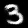
\includegraphics[scale=2.0]{images/rand_gen1}
		\end{subfigure}
		\begin{subfigure}[b]{0.2\textwidth}
			\centering
			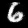
\includegraphics[scale=2.0]{images/rand_gen2}
		\end{subfigure}		
		\begin{subfigure}[b]{0.2\textwidth}
			\centering
			
\includegraphics[scale=2.0]{images/rand_gen3}
		\end{subfigure}
		\begin{subfigure}[b]{0.2\textwidth}
			\centering
			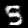
\includegraphics[scale=2.0]{images/rand_gen5}
		\end{subfigure}
		
		\caption{Images generated from random input vectors.}
		\label{fig:random_generated}
	\end{figure} 

	\subsubsection{Unlabeled Data}
	Using unlabeled data during unsupervised pretraining can be very useful if you do not have much labeled data available for your particular problem. To simulate this scenario I randomly selected 5000 images from the MNIST training set to use as labeled data and left the remaining images as unlabeled. 
	
	I pretrained the DBN using the ``unlabeled'' data and then ran standard backpropagation using the 5000 labeled images. For comparison I initialized an MLP with the same number of nodes and layers as the DBN and trained it using only the labeled data. Even with the small training set the pretrained DBN achieved a final accuracy of 91.3\%, greatly outperforming the basic MLP which had a final accuracy of only 56.1\%.  
	
	Under the conditions described in the previous experiments the DBN  often tied the MLP baseline in final accuracy but never outperformed it. In this case, however, the DBN was much more resilient to the shrinking of the training dataset than the MLP thanks to its ability to use unlabeled data.
	
	\section{Conclusion}
	
	
	
\end{document}